\chapter{Principles}

This chapter describes basic informations about radiation environment, failure modes in electronic devices and introduction to RadFET dosimetry.

\section{Radiation on Low Earth Orbit}
    Radiation on LEO comes from trapped particle belts, solar particle events and cosmic rays \cite{ESA_radiation}. There are also other sources of radiation, but they are negligible comparing to those effects.

    \bigskip \textbf{Trapped particles}

    Electrons and protons are being trapped in Earth's magnetic field, following magnetic fields lines. They are serious concern on Low Earth Orbit along polar regions and inside South Atlantic Anomaly. In the figure \ref{Polar_SAA} radiation pattern along Earth is shown.

    \begin{figure}[H]
        \centering
        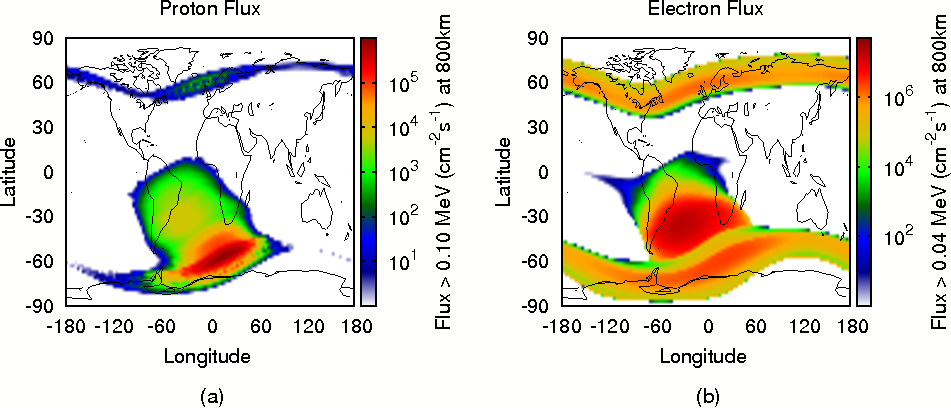
\includegraphics[width=0.8\paperwidth]{img/03/polar_SAA.png}
        \caption{Radiation pattern on LEO. Source: \cite{ESA_radiation}}
        \label{Polar_SAA}
    \end{figure}

    \bigskip \textbf{Solar flares}

    During solar flares large fluxes of protons are produced, and some of them are reaching Earth. Magnetic field provides shielding from them, but they are being trapped in it, easily reaching polar regions and South Atlantic Anomaly. Solar flares are unpredictable, being a threat to spacecraft operations.

    \bigskip \textbf{Cosmic rays}

    Cosmic rays originates from outside the solar system. They are very high energy particles, which make shielding very difficult. Flux of this kind of particles is low, therefore they mostly contribute in single-event processes.

\section{Radiation effects on electronic devices}
    There are two basic effects of radiation on silicon components:
    \begin{itemize}
        \item ionizing effect
        \item displacement damage
    \end{itemize}

    Those two effect are responsible for changing parameters of semiconductor devices, which after some time can lead to failure of the device. Main source of this radiation are gamma (ionization) and neutron particles (displacement).

    In space electronics during analysis and design two major problems are considered - Single Event Effects (SEE) and Total Ionizing Dose (TID). Every silicon and silica device is susceptible to both of those - and both have to be considered during product design, development and testing.

    \subsection{Single Events Effects}
        Single Event Effects are connected with generation of electron-hole pair in semiconductor, when material is exposed to ionizing radiation. Amount of pairs generated is proportional to energy deposited. For semiconductor device parameter $LET_{th}$ (Linear Energy Transfer Threshold) is defined, being a measure of how susceptible the device is. For particles with Linear Energy Transfer (LET - normalized particle energy per mass of the absorbing material), below this threshold no effect will be observed.

        Single Event Effects are divided into two groups - non-destructive (fully recoverable, possibly after power cycle) and destructive (permanent damage) effects. Shortly those are described below, defined as in \cite{ECSS_Q_ST_60_15C}.

        \bigskip\textbf{Non-destructive effects}
        \begin{itemize}
            \item \textbf{Single Event Upset} - especially memory-based devices (like microprocessors, memories, Field Programmable Gate Array - FPGA) are vulnerable. This phenomenon will possibly alter the state of cell in memory - causing memory corruption. This can lead to complete failure of device if this is not corrected.

            \item \textbf{Single Event Functional Interrupt} - subset of SEU - this effect cause the system to latch in non-recoverable state (e.g. by switching to wrong state in state machine). Only option is to reset circuit to back to known state.

            \item \textbf{Single Event Transient} - are formed as a voltage/current spurious pulses generated by charge induced by striking particle. This can cause different problems - from disturbing analog electronics up to causing switch of digital circuit. This effect strongly depends on size of feature in silica.
        \end{itemize}

        \bigskip\textbf{Destructive effects}
        \begin{itemize}
            \item \textbf{Single Event Latch-up} - particle striking can cause turning on parasitic thyristor in CMOS structure. This will lead to effectively shorting voltage supply to ground, causing overheat and damage to the device.

            \item \textbf{Single Event Gate Rupture} - high energy particle comes through thin gate (especially in MOS transistors) can cause generation of electron-holes pairs in gate and substrate - causing high electric field across gate. When this effect is strong enough it can cause permanent damage to transistor.

            \item \textbf{Single Event Burnout} - ion that traverses the transistor structure (through the source) can induce a current flow that turns on the parasitic npn transistor. This leads to effective short circuit and damage to the device.
        \end{itemize}

        \bigskip\textbf{Mitigation techniques}

        Below recommended mitigation techniques for SEE were listed:
        \begin{itemize}
            \item SEU - redundancy, memory scrubbing,
            \item SEFI - watchdog, proper reset sequence,
            \item SET - use lower-integration scale devices, implement protection resistors etc.
            \item SEL - implement overcurrent circuits (like Latch-up Current Limiters),
            \item SEGR, SEB - use higher $LET_{th}$ devices
        \end{itemize}

    \subsection{Total Ionizing Dose}
        TID is defined as total energy absorbed during exposure. This can be caused by any kind of radiation, behaving differently in every semiconductor device. In general, TID successively degrades electronic device parameters in time, causing them to stop functioning when critical irradiation was reached. Effect in p-MOSFET transistor is described in section \ref{Radiation_effects_on_MOS_transistors}.

\section{Need for TID radiation dosimetry}
    During spacecraft mission accumulated radiation level should be monitored to not excess guaranteed values for components. For example, near end of its lifetime, spacecraft can be commanded to deorbit into atmosphere or move to graveyard orbit - before fail can occur, causing losing control of spacecraft, like for example in Telstar-1.
    Absorbed dose simulation is good method of its estimation. But, because radiation flux changes (due to cosmic event, like solar flares) errors can accumulate during satellite lifetime. Flying by South Atlantic Anomaly or Van Allen belts can cause radiation estimation to be inaccurate, so near all spacecrafts implement sensor which constantly monitor radiation level absorbed by its electronics.

\section{On-line TID radiation dosimetry}
    Couple of possible dosimetry methods were considered:
    \begin{itemize}
        \item PIN diode - forward voltage shift during irradiation \cite{PIN_dosimetry},
        \item memory dosimetry - single events cause bit flips in memory - accumulated number of errors reflects absorbed dose \cite{RadFET_PhD},
        \item FGMOSFET - change in differential channel current - indicative of radiation dose \cite{FGMOSFET_patent},
        \item RadFET - shift of threshold voltage of p-MOS transistor indicates irradiation \cite{RadFET_PhD}.
    \end{itemize}
    Detailed description of those dosimetry methods can be found in \cite{RadFET_PhD}.

    For this sensor, it was decided to use RadFET as a sensing element. This kind of sensors have already flown on many satellites, are used in medical and industrial dosimetry.

    The most important advantages of RadFET dosimetry:
    \begin{itemize}
        \item sensor can be completely shut down during irradiation (no power consumption and increased reliability),
        \item integrated measurement (especially important for small dose rates),
        \item on-line, non-destructive readout,
        \item small size,
    \end{itemize}
    And most crucial drawbacks:
    \begin{itemize}
        \item low sensitivity - requires sophisticated measurement setup,
        \item required temperature compensation.
    \end{itemize}


\section{RadFET Theory}
    Basic idea of RadFET of using metal-oxide semiconductor field-effect transistor (MOSFET) is to measure its threshold voltage shift, $\Delta V_{TH}$ and covert it into absorbed dose.

    \subsection{Radiation effects on MOS transistors}
    \label{Radiation_effects_on_MOS_transistors}
        Irradiation of MOSFET transistor results in threshold voltage shift. It is caused by trapping of holes (generated during particle strike) and creation of interface states on gate/bulk boundary. Those effects are shown in the figure \ref{MOS_irradiation} \cite{pMOS_dosimeters_radfets}.

        \begin{figure}[H]
            \centering
            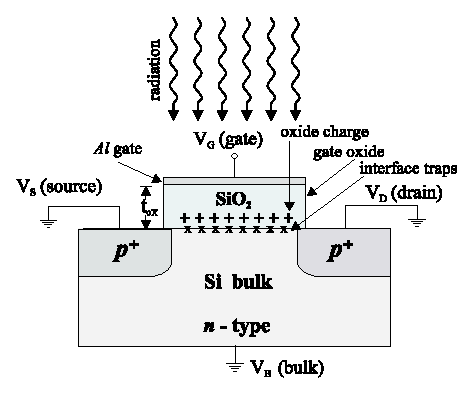
\includegraphics[width=0.4\paperwidth]{img/03/MOS_irradiation_schematic.eps}
            \caption{pMOS irradiation schematic. Source: \cite{pMOS_dosimeters_radfets}}
            \label{MOS_irradiation}
        \end{figure}

        Threshold voltage will shift according to following equation \cite{pMOS_dosimeters_radfets}:

        $$\Delta V_{TH} = A \cdot D^n$$

        Where:

        \begin{tabular}{lcl}
            $\Delta V_{TH}$ & - & threshold voltage shift \\
            $A$ & - & constant \\
            $D$ & - & absorbed dose \\
            $n$ & - & degree of linearity (ideally $n = 1$) \\
        \end{tabular}
        \bigskip



    \subsection{Threshold voltage measurement}
        Simplest method to measure threshold voltage shift is to use diode configuration of MOS transistor, current source and measure voltage across, as shown in the figure \ref{MOS_measurement_setup}.

        \begin{figure}[H]
            \centering
            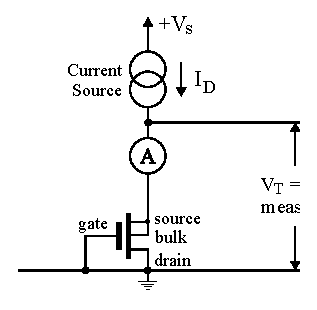
\includegraphics[width=0.3\paperwidth]{img/03/Vth-measurement-setup.eps}
            \caption{Measurement setup. Source: \cite{pMOS_dosimeters_radfets}}
            \label{MOS_measurement_setup}
        \end{figure}

    \subsection{Temperature dependencies}
        Threshold voltage of transistor strongly depends on die temperature \cite{managing_temperature_effects_in_nanoscale_adaptive_systems}.

        This dependency is usually described to be linear:

        $$\Delta V_{TH} = A \cdot \Delta T$$

        Where:

        \begin{tabular}{lcl}
            $\Delta V_{TH}$ & - & threshold voltage shift \\
            $A$ & - & constant \\
            $\Delta T$ & - & temperature change \\
        \end{tabular}
        \bigskip

        Constant coefficient depends on particular MOSFET, technology and (very weak effect) irradiation. Usually this coefficient is in range $-0.1$ to \SI{-1}{\milli\volt/\kelvin}.
